\documentclass[12pt]{article}

\usepackage{algorithm} %pseudo-code
\usepackage{algpseudocode}
\usepackage[top=1in, bottom=1in, left=1in, right=1in]{geometry}
\usepackage{amsmath,amsthm,amssymb}
\usepackage{graphicx}
\usepackage{float}
\usepackage{amsmath, amssymb, amscd}
\usepackage{alltt}
\usepackage{textcomp}
\usepackage{gensymb}
\usepackage{multicol}
\usepackage{tabularx}

\newcommand{\N}{\mathcal{N}}
\newcommand{\Z}{\mathbb{Z}}
\newcommand{\R}{\mathbb{R}}
\newcommand{\bigo}{\mathcal{O}}
\newcommand{\G}{\mathcal{G}}
\newcommand{\V}{\mathcal{V}}
\newcommand{\E}{\mathcal{E}}
\newcommand{\K}{\mathcal{K}}
\newcommand{\T}{^\intercal}

\newcommand{\sups}[1]{\ensuremath{^{\textrm{#1}}}}
\newcommand{\subs}[1]{\ensuremath{_{\textrm{#1}}}}

\newcommand{\specialcell}[2][c]
{
  \begin{tabular}[#1]{@{}c@{}}#2\end{tabular}
}

\makeatletter
\newsavebox{\mybox}\newsavebox{\mysim}
\newcommand{\distras}[1]
{
  \savebox{\mybox}{\hbox{\kern3pt$\scriptstyle#1$\kern3pt}}%
  \savebox{\mysim}{\hbox{$\sim$}}%
  \mathbin{\overset{#1}{\kern\z@\resizebox{\wd\mybox}{\ht\mysim}{$\sim$}}}%
}
\makeatother
\makeatletter
\renewcommand*\env@matrix[1][c]{\hskip -\arraycolsep
  \let\@ifnextchar\new@ifnextchar
  \array{*\c@MaxMatrixCols #1}}
\makeatother
%===============================================================================
% code highlighting :
\usepackage{listings}

% define custom colors :
\usepackage{color}
\definecolor{bg}{rgb}{0.96,0.96,0.85}
\definecolor{deepblue}{rgb}{0,0,0.5}
\definecolor{deepred}{rgb}{0.6,0,0}
\definecolor{deepgreen}{rgb}{0,0.5,0}

\usepackage{xcolor}
\renewcommand{\lstlistlistingname}{Code Listings}
\renewcommand{\lstlistingname}{Code Listing}
\definecolor{gray}{gray}{0.5}
\colorlet{commentcolour}{green!50!black}

\colorlet{stringcolour}{red!60!black}
\colorlet{keywordcolour}{magenta!90!black}
\colorlet{exceptioncolour}{yellow!50!red}
\colorlet{commandcolour}{blue!60!black}
\colorlet{numpycolour}{blue!60!green}
\colorlet{literatecolour}{magenta!90!black}
\colorlet{promptcolour}{green!50!black}
\colorlet{specmethodcolour}{violet}
\colorlet{indendifiercolour}{green!70!white}

\newcommand{\framemargin}{5ex}

\newcommand{\literatecolour}{\textcolor{literatecolour}}

\newcommand\pythonstyle{\lstset{
%keepspaces=true,
language=python,
showtabs=true,
tab=,
tabsize=2,
basicstyle=\ttfamily\scriptsize,%\setstretch{.5},
stringstyle=\color{stringcolour},
showstringspaces=false,
alsoletter={1234567890},
otherkeywords={\ , \}, \{, \%, \&, \|},
keywordstyle=\color{keywordcolour}\bfseries,
emph={and,break,class,continue,def,yield,del,elif ,else,%
except,exec,finally,for,from,global,if,import,in,%
lambda,not,or,pass,print,raise,return,try,while,assert},
emphstyle=\color{blue}\bfseries,
emph={[2]True, False, None},
emphstyle=[2]\color{keywordcolour},
emph={[3]object,type,isinstance,copy,deepcopy,zip,enumerate,reversed,list,len,dict,tuple,xrange,append,execfile,real,imag,reduce,str,repr},
emphstyle=[3]\color{commandcolour},
emph={Exception,NameError,IndexError,SyntaxError,TypeError,ValueError,OverflowError,ZeroDivisionError},
emphstyle=\color{exceptioncolour}\bfseries,
%upquote=true,
morestring=[s]{"""}{"""},
morestring=[s]{'''}{'''},
commentstyle=\color{commentcolour}\slshape,
%emph={[4]1, 2, 3, 4, 5, 6, 7, 8, 9, 0},
emph={[4]ode, fsolve, sqrt, exp, sin, cos, arccos, pi,  array, norm, solve, dot, arange, , isscalar, max, sum, flatten, shape, reshape, find, any, all, abs, linspace, legend, quad, polyval,polyfit, hstack, concatenate,vstack,column_stack,empty,zeros,ones,rand,vander,grid,pcolor,eig,eigs,eigvals,svd,qr,tan,det,logspace,roll,min,mean,cumsum,cumprod,diff,vectorize,lstsq,cla,eye,xlabel,ylabel,squeeze,plot,median,std,hist},
emphstyle=[4]\color{numpycolour},
emph={[5]__init__,__add__,__mul__,__div__,__sub__,__call__,__getitem__,__setitem__,__eq__,__ne__,__nonzero__,__rmul__,__radd__,__repr__,__str__,__get__,__truediv__,__pow__,__name__,__future__,__all__},
emphstyle=[5]\color{specmethodcolour},
emph={[6]assert,range,yield},
emphstyle=[6]\color{keywordcolour}\bfseries,
% emph={[7]self},
% emphstyle=[7]\bfseries,
literate=*%
{:}{{\literatecolour:}}{1}%
{=}{{\literatecolour=}}{1}%
{-}{{\literatecolour-}}{1}%
{+}{{\literatecolour+}}{1}%
{*}{{\literatecolour*}}{1}%
{/}{{\literatecolour/}}{1}%
{!}{{\literatecolour!}}{1}%
%{(}{{\literatecolour(}}{1}%
%{)}{{\literatecolour)}}{1}%
{[}{{\literatecolour[}}{1}%
{]}{{\literatecolour]}}{1}%
{<}{{\literatecolour<}}{1}%
{>}{{\literatecolour>}}{1}%
{>>>}{{\textcolor{promptcolour}{>>>}}}{1}%
,%
breaklines=true,
breakatwhitespace= true,
%xleftmargin=\framemargin,
%xrightmargin=\framemargin,
aboveskip=1ex,
frame=trbl,
%frameround=tttt,
rulecolor=\color{black!40},
%framexleftmargin=\framemargin,
%framextopmargin=.1ex,
%framexbottommargin=.1ex,
%framexrightmargin=\framemargin,
%framexleftmargin=1mm, framextopmargin=1mm, frame=shadowbox, rulesepcolor=\color{blue},#1
%frame=tb,
backgroundcolor=\color{yellow!10}
}}

% Python environment
\lstnewenvironment{python}[1][]
{
  \pythonstyle
  \lstset{#1}
}
{}

% Python for external files
\newcommand\pythonexternal[1]
{{
  \pythonstyle
  \lstinputlisting{#1}
}}

% Python for inline
\newcommand\pythoninline[1]{{\pythonstyle\lstinline!#1!}}

% end code highlighting
%===============================================================================

\DeclareMathOperator*{\argmax}{arg\,max}

\usepackage[top=.5in, bottom=1in, left=.75in, right=.75in]{geometry}
\usepackage{framed}
\definecolor{shadecolor}{gray}{0.9}
\setlength{\columnsep}{8mm}

\begin{document}
\small
\twocolumn

\title{Project 05 - Bayes Network}
\author{Evan Cummings\\
CSCI 544 - Machine Learning}

\maketitle

\section{Program usage}

In the \texttt{src} folder, simply type

\centerline{\texttt{python bayes\_network.py}}

\noindent which results in the output

\begin{shaded}
\tiny
\begin{alltt}
FOLD 1
-----------------------------------------------------------
Node : Storms   Parent of Storms : []
Node : BusTourGroup   Parent of BusTourGroup : []
Node : Lightning  Parent of Lightning : ['Storms']
Node : Campfire   Parent of Campfire : ['BusTourGroup', 'Storms']
Node : Thunder  Parent of Thunder : ['Lightning']

FOLD 2
-----------------------------------------------------------
Node : Storms   Parent of Storms : []
Node : BusTourGroup   Parent of BusTourGroup : []
Node : Lightning  Parent of Lightning : ['Storms']
Node : Campfire   Parent of Campfire : ['BusTourGroup', 'Storms']
Node : Thunder  Parent of Thunder : ['Lightning']

FOLD 3
-----------------------------------------------------------
Node : Storms   Parent of Storms : []
Node : BusTourGroup   Parent of BusTourGroup : []
Node : Lightning  Parent of Lightning : ['Storms']
Node : Campfire   Parent of Campfire : ['BusTourGroup', 'Storms']
Node : Thunder  Parent of Thunder : ['Lightning']

FOLD 4
-----------------------------------------------------------
Node : Storms   Parent of Storms : []
Node : BusTourGroup   Parent of BusTourGroup : []
Node : Lightning  Parent of Lightning : ['Storms']
Node : Campfire   Parent of Campfire : ['BusTourGroup', 'Storms']
Node : Thunder  Parent of Thunder : ['Lightning']

FOLD 5
-----------------------------------------------------------
Node : Storms   Parent of Storms : []
Node : BusTourGroup   Parent of BusTourGroup : []
Node : Lightning  Parent of Lightning : ['Storms']
Node : Campfire   Parent of Campfire : ['BusTourGroup', 'Storms']
Node : Thunder  Parent of Thunder : ['Lightning']

FOLD 6
-----------------------------------------------------------
Node : Storms   Parent of Storms : []
Node : BusTourGroup   Parent of BusTourGroup : []
Node : Lightning  Parent of Lightning : ['Storms']
Node : Campfire   Parent of Campfire : ['BusTourGroup', 'Storms']
Node : Thunder  Parent of Thunder : ['Lightning']

FOLD 7
-----------------------------------------------------------
Node : Storms   Parent of Storms : []
Node : BusTourGroup   Parent of BusTourGroup : []
Node : Lightning  Parent of Lightning : ['Storms']
Node : Campfire   Parent of Campfire : ['BusTourGroup', 'Storms']
Node : Thunder  Parent of Thunder : ['Lightning']

FOLD 8
-----------------------------------------------------------
Node : Storms   Parent of Storms : []
Node : BusTourGroup   Parent of BusTourGroup : []
Node : Lightning  Parent of Lightning : ['Storms']
Node : Campfire   Parent of Campfire : ['BusTourGroup', 'Storms']
Node : Thunder  Parent of Thunder : ['Lightning']

FOLD 9
-----------------------------------------------------------
Node : Storms   Parent of Storms : []
Node : BusTourGroup   Parent of BusTourGroup : []
Node : Lightning  Parent of Lightning : ['Storms']
Node : Campfire   Parent of Campfire : ['BusTourGroup', 'Storms']
Node : Thunder  Parent of Thunder : ['Lightning']

FOLD 10
-----------------------------------------------------------
Node : Storms   Parent of Storms : []
Node : BusTourGroup   Parent of BusTourGroup : []
Node : Lightning  Parent of Lightning : ['Storms']
Node : Campfire   Parent of Campfire : ['BusTourGroup', 'Storms']
Node : Thunder  Parent of Thunder : ['Lightning']

percent correct: 99.3%
\end{alltt}
\small
\end{shaded}

This shows the parents of each node of the resulting DAG derived from 10-fold cross-validation on the forest fire data included in the \texttt{data} directory.  The final accuracy is reported on the last line.

\section{Data}

\begin{figure}[H]
  \centering
		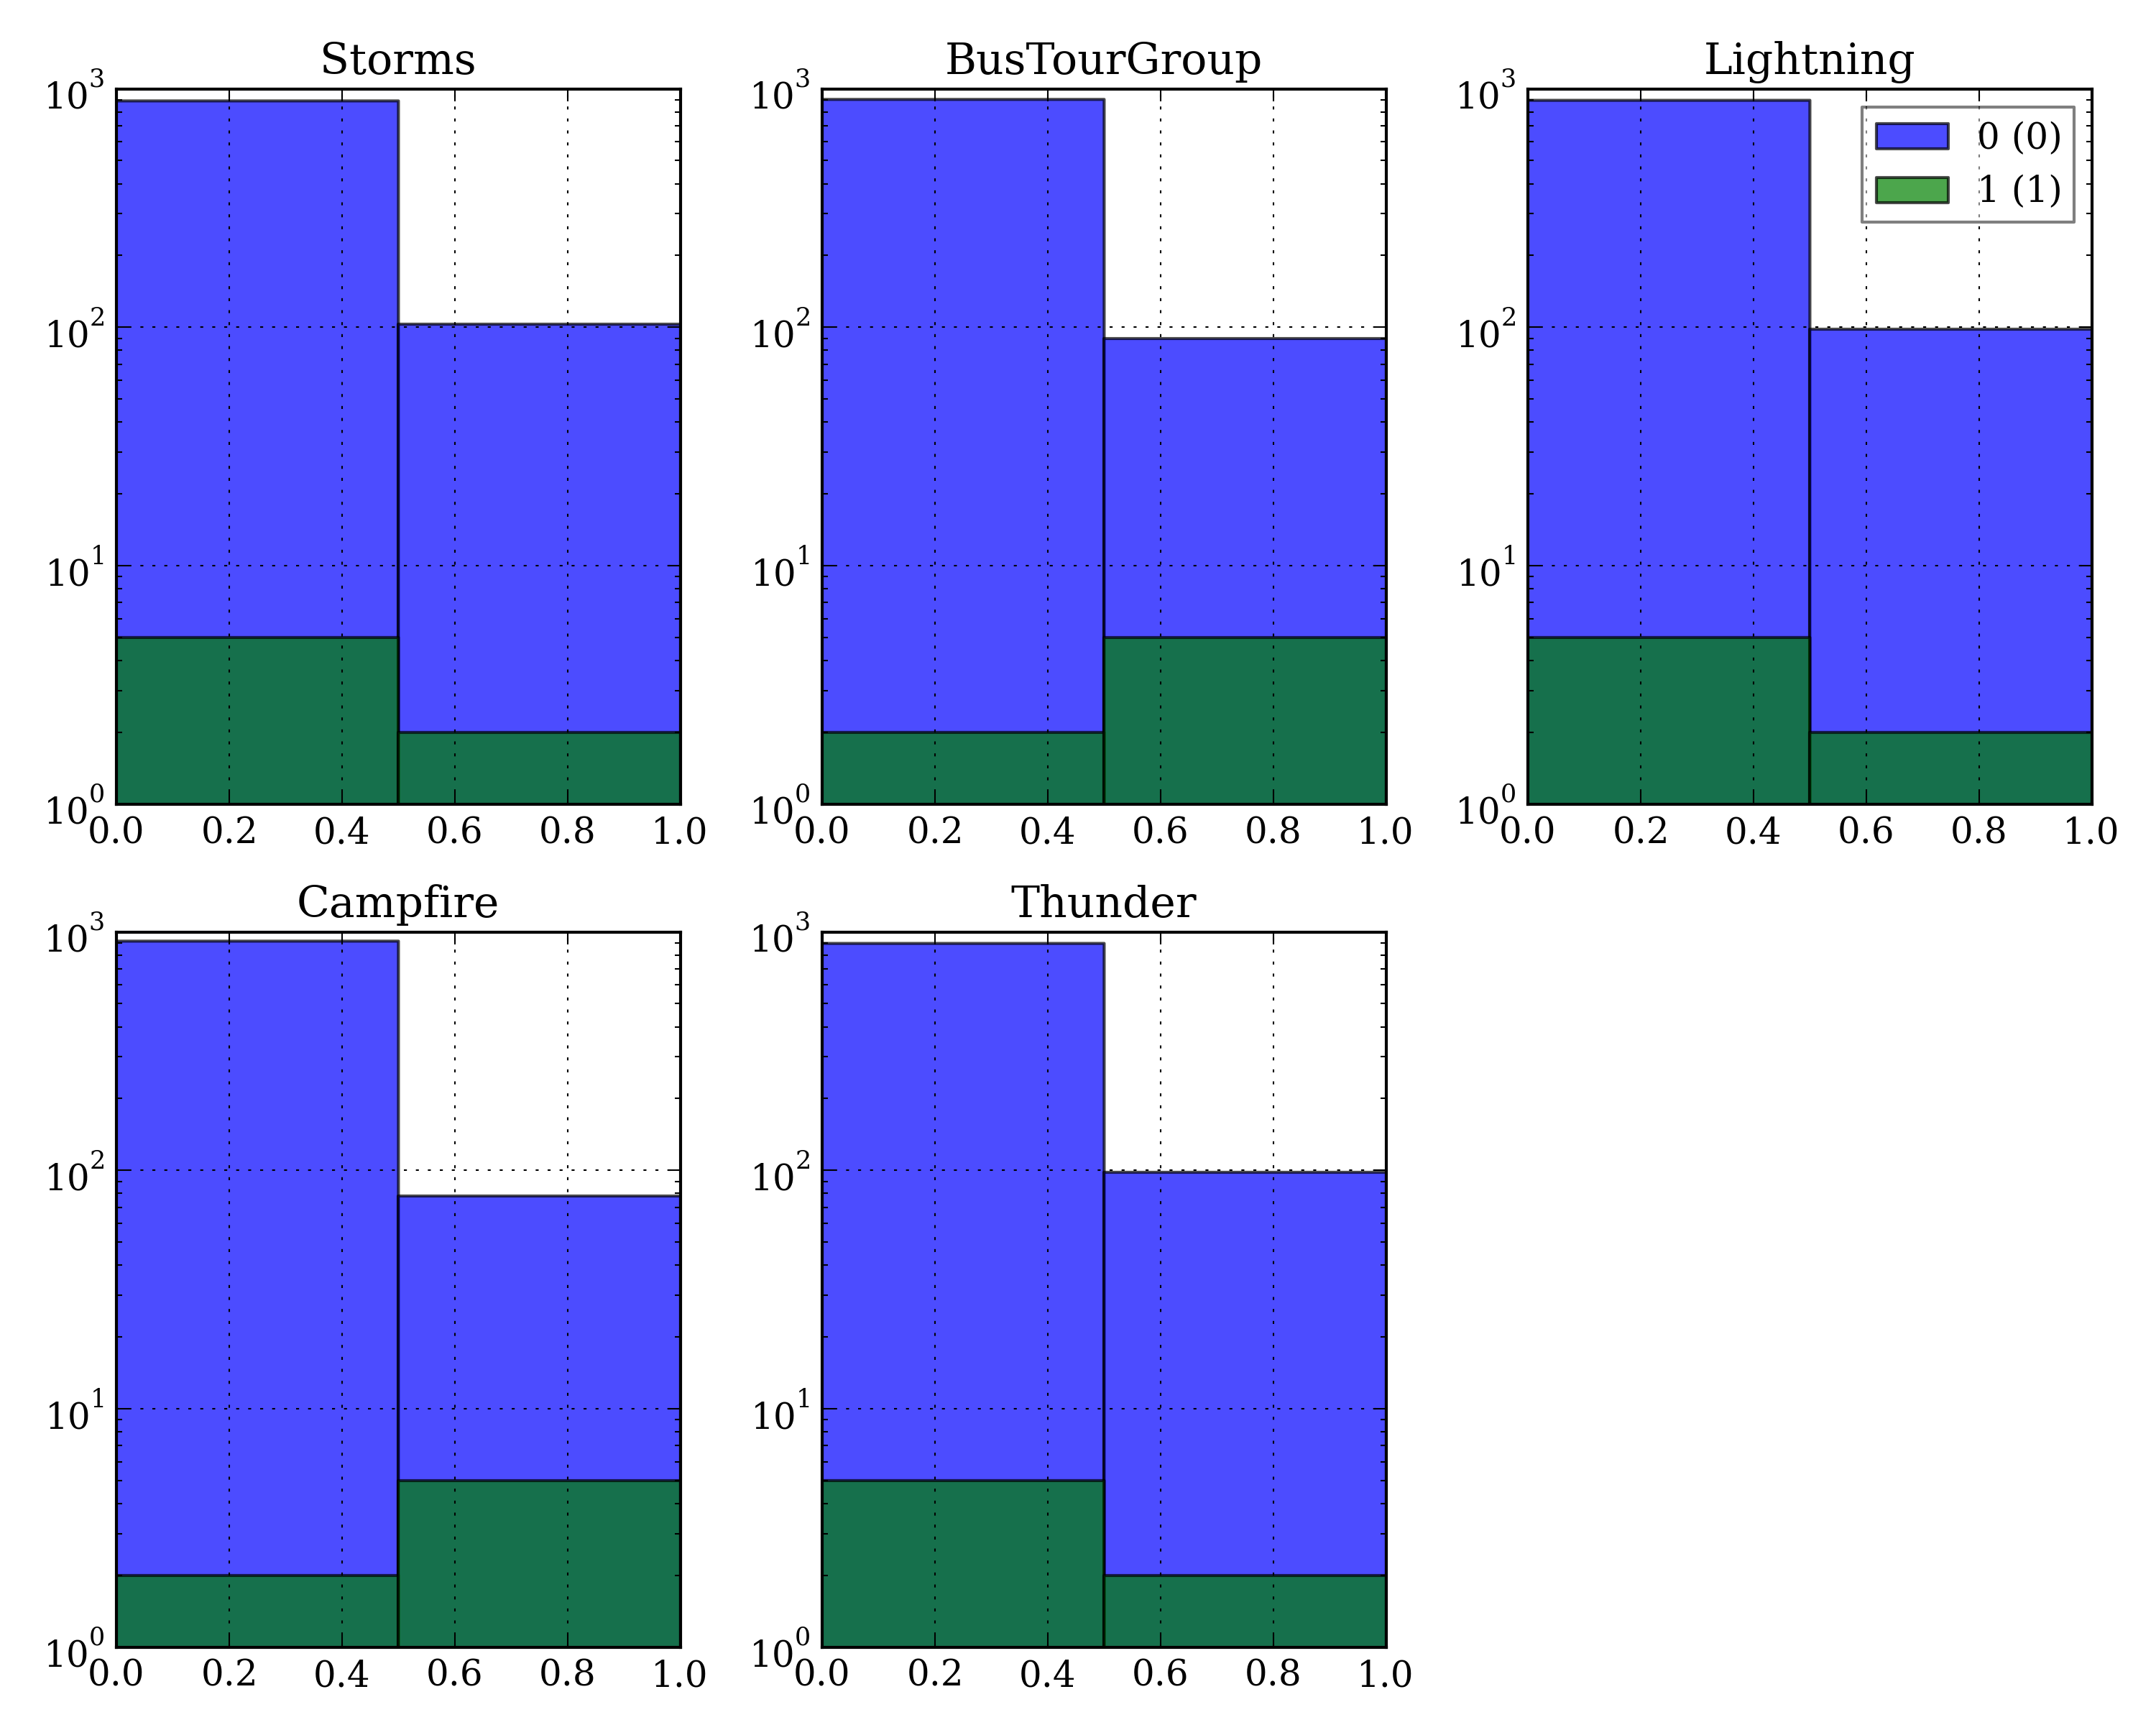
\includegraphics[width=0.4\textwidth]{images/data.png}
  \caption{\scriptsize The data for the project, separated by dimension.  Note that there are far more negative (0) entries than positive (1) in all dimensions.}
\end{figure}
 

\end{document}




